\chapter{Acoustic radiation force over a cylinder and a sphere}

\begin{figure*}
    \begin{subfigure}{0.4\textwidth}
    \centering
    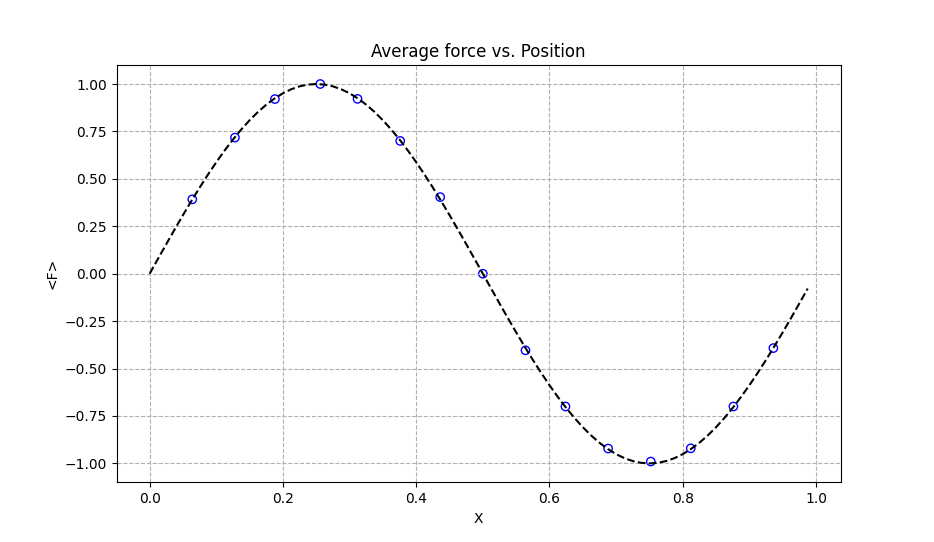
\includegraphics[width=\textwidth]{images/Results/Position2D.png}
    \caption{Dependence of the force on position.}
    \label{fig:position}
    \end{subfigure}
    \begin{subfigure}{0.35\textwidth}
    \centering
    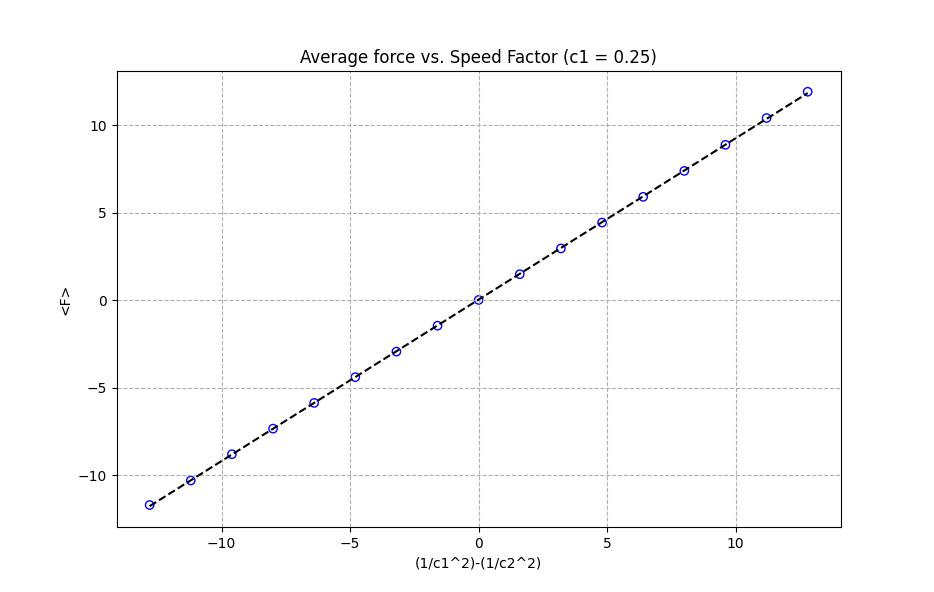
\includegraphics[width=\textwidth]{images/Results/Speed_C1_025.png}
    \caption{Cubic relation between the force and radius.}
    \label{fig:radius}
    \end{subfigure}
    \begin{subfigure}{0.4\textwidth}
    \centering
    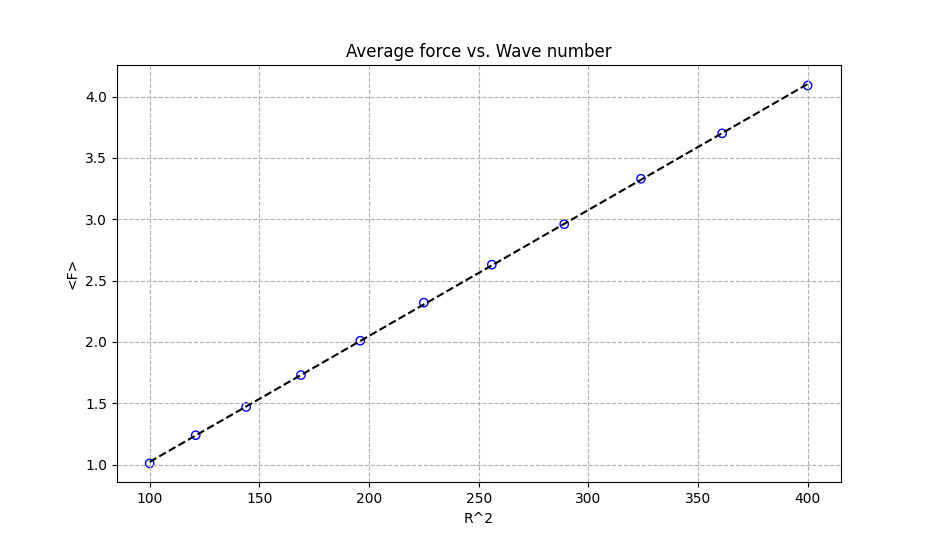
\includegraphics[width=\textwidth]{images/Results/radius2D.png}
    \caption{Dependence of the force on squared radius.}
    \label{fig:position}
    \end{subfigure}
    \begin{subfigure}{0.35\textwidth}
    \centering
    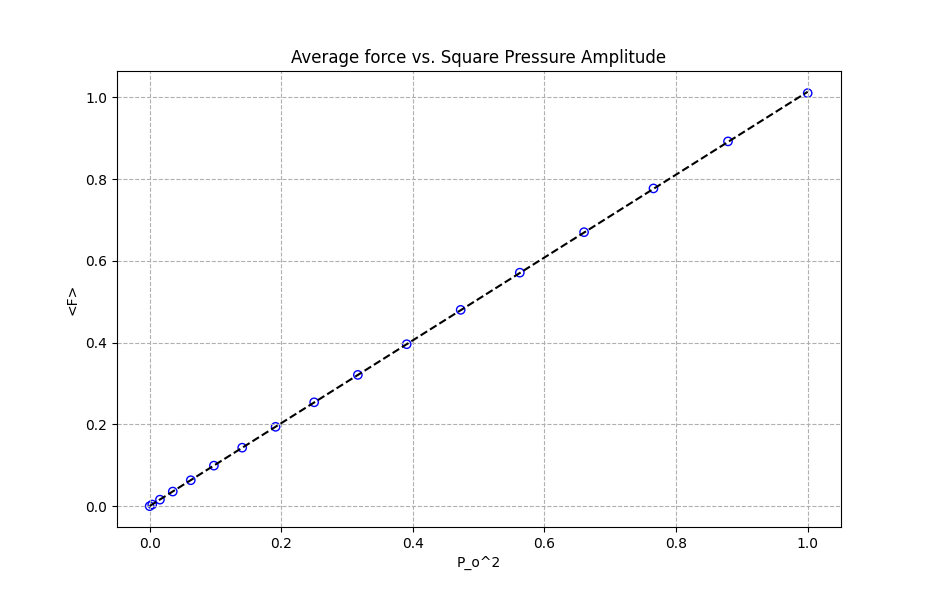
\includegraphics[width=\textwidth]{images/Results/Amplitude2D.png}
    \caption{Dependence of the force on squared pressure Amplitude.}
    \label{fig:radius}
    \end{subfigure}
    \begin{subfigure}{0.35\textwidth}
    \centering
    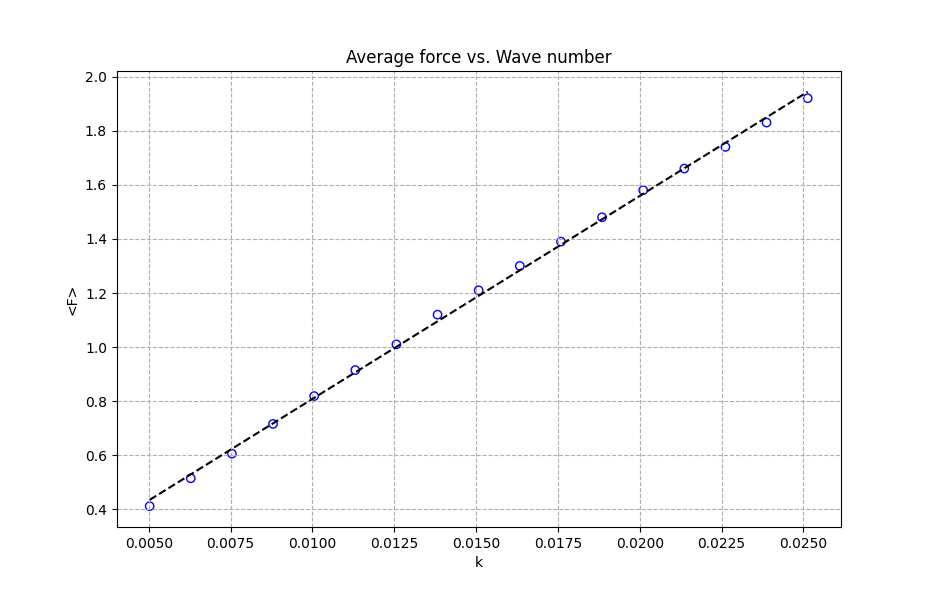
\includegraphics[width=\textwidth]{images/Results/WaveNumber2D.png}
    \caption{Dependence relation with wave number.}
    \label{fig:radius}
    \end{subfigure}
    \caption{Compilation of results of the acoustic radiation force.}
    \label{fig:ARF_results}
\end{figure*}


Numerical simulations were made to produce consistent results with the experiment. The very first step was to familiarize with the LB3D code, reading all the available documentation and asking to the development team about the features and logic of the code. The documentation available is not enough to understand the use of it, so it was necessary to clarify many questions during office hours. This led to show the purpose of the work and solve struggles faced during the compilation and execution of the tests. The very first test done was to implement the Lattice Boltzmann model for waves explained in section \ref{sec:LBW}. During this implementation the following tests were done: A Gaussian pulse propagated in space by imposing an initial condition, a point source of waves imposing the pressure at a single point in space, and the generation of standing waves from a source of plane waves. The idea was to compare the output of two codes, one is a standard implementation in C++ and the other one was made in LB3D. In the figures \ref{fig:gauss_init} and \ref{fig:gauss_final} shows the output generated by both codes, one as the initial state and the other at a final state respectively. In the figure \ref{fig:point_source} the comparison between the output of both codes is gotten, and at the left the comparison of the density at the x-axis of both outputs and the theoretical solution. With these tests it was possible to confirm that the implementation of LB3D was successful. 

Another result reached, which is relevant for the objectives of the project, was the production of standing waves by imposing a source wall and a reflective wall at the left of a simulation box domain. This was produced by using the equations written in \ref{eq:imposing_source} and two solid walls that reflect the wave back and for and dissipate a bit. This will produce a resonator with standing waves useful to build the simulation of a sphere under a pressure field. A capture of this result can be seen in the figure \ref{fig:standing-waves},  where the steady state has been reached. In order to simulate the boundary conditions for refraction and reflection, another simulation was performed where an plane interphase was placed at the middle of a one-dimensional box. The interphase separates two regions: One with a propagation speed of 0.5 cells per timestep and the other one with 0.25 cells per timesteps. The result can be seen in figure \ref{fig:interphase} where two moments in time show the ongoing wave before entering the interphase and then after entering the interphase a reflected and transmitted pulse was propagated.
This simulation was totally necessary in order to be sure that the boundary conditions are satisfied properly. This will produce a scattered reflected field able to produce a non-linear acoustic force which acts in the time average of acoustic oscillations. In the LB3D code there is a possibility to include mesh objects that are affected by the fluid. The code was modified in order to be affected instead by an acoustic field, such that the force written in \ref{eq:arf_integral} was successfully computed. This implementation was not easy to do and it did cost an entire month of development and assistance with the development team. Finally the results were obtained in a satisfactory way. The comparison with the analytical solution for the Gorkov acoustic radiation force was done in a bi-dimensional case and the relationships with the physical variables made a good agreement between the numerical result and the theoretical model. Some of the results of the figure \ref{fig:ARF_results} are shown as linear fits of the corresponding variables of the equation \ref{eq:ARF_Gorkov_3D} as the pressure amplitude, the wave number, the densities and sound speeds of both the fluid and the object, and the size of the object. This force is proportional to the cube of the radius as seen in \ref{fig:radius}, also increases linearly with the wave number (see fig. \ref{fig:wavenumber}) and with the square of the pressure amplitude as it's shown in the figure \ref{fig:amplitude}. Also, in the figure \ref{fig:position} is shown how the force is dependent of position, such that in the pressure node this force will be zero and the object will be confined in the node, thus, the effect of acoustic levitation was simulated successfully. This results shows that it have been possible to reproduce a simulation with the acoustic radiation force in a general way, where an acoustic field is able to affect this object in the time average. 

These are the results of four months of work, but the project have been continuing and providing more results that have been developed after the research stay. This project is currently in development and the nex step is to make the simulation of a magnetic rotor composed by tiny spheres which moves along an acoustic fields and it experience rolling under the influence of a rotating external and uniform magnetic field. The results shown in this document are the summary of more results which will be soon published as a scientific paper. The plans about this publication process are under discussion with the supervisors.

\begin{figure*}
    \begin{subfigure}{0.4\textwidth}
    \centering
    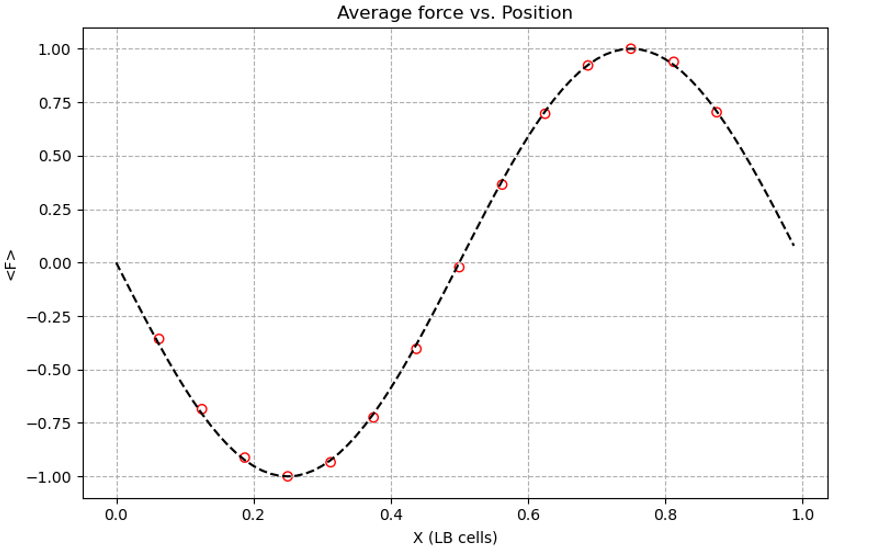
\includegraphics[width=\textwidth]{images/Results/Position.PNG}
    \caption{Dependance of the force on position.}
    \label{fig:position}
    \end{subfigure}
    \begin{subfigure}{0.35\textwidth}
    \centering
    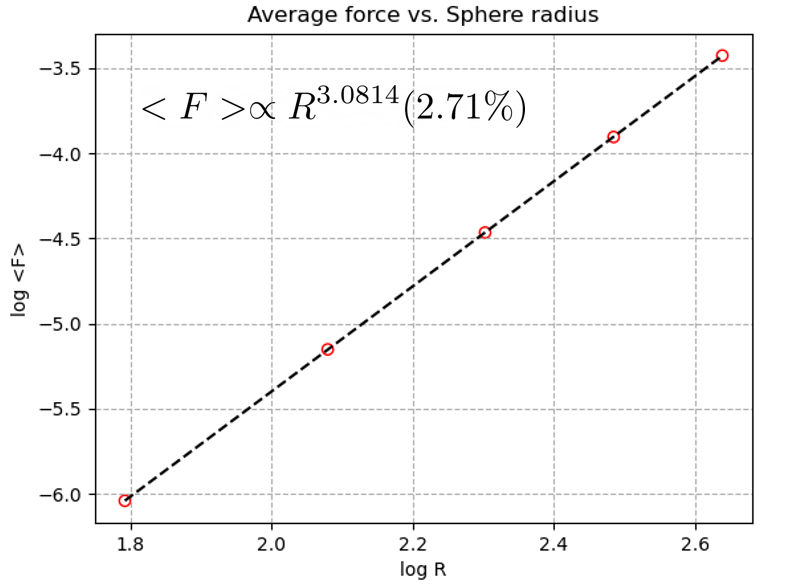
\includegraphics[width=\textwidth]{images/Results/Radius.PNG}
    \caption{Relation between the force and sound speed with medium speed $c_1=0.25$.}
    \label{fig:radius}
    \end{subfigure}
    \begin{subfigure}{0.4\textwidth}
    \centering
    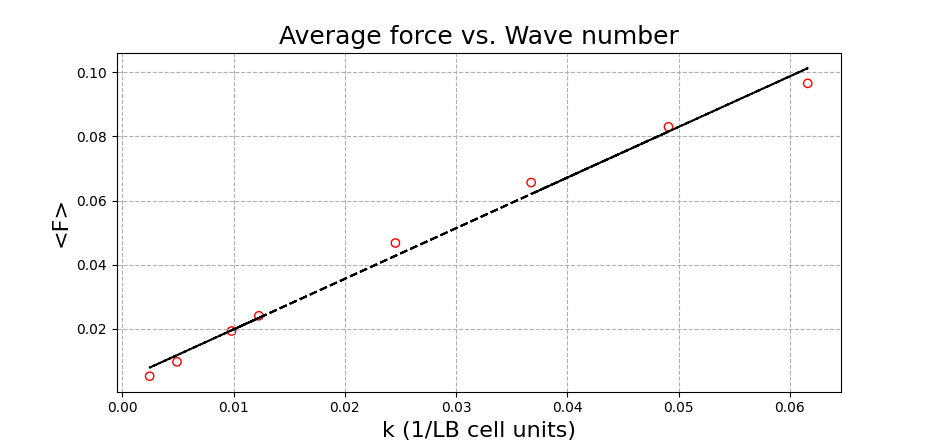
\includegraphics[width=\textwidth]{images/Results/ResultWaveNumber.PNG}
    \caption{Linear relation between the force and the wave number.}
    \label{fig:wavenumber}
    \end{subfigure}
    \begin{subfigure}{0.35\textwidth}
    \centering
    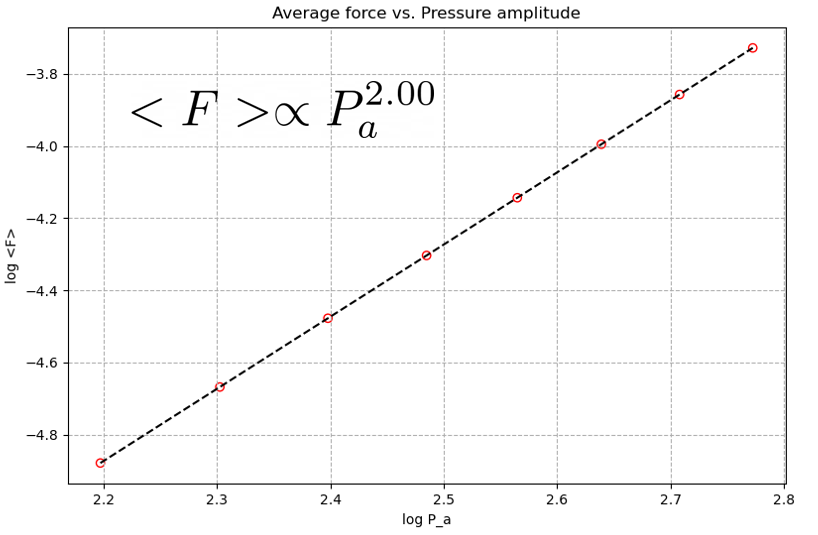
\includegraphics[width=\textwidth]{images/Results/PressureAmplitude.PNG}
    \caption{Cuadratic relation between the force and the pressure amplitude.}
    \label{fig:amplitude}
    \end{subfigure}
    \begin{subfigure}{0.4\textwidth}
    \centering
    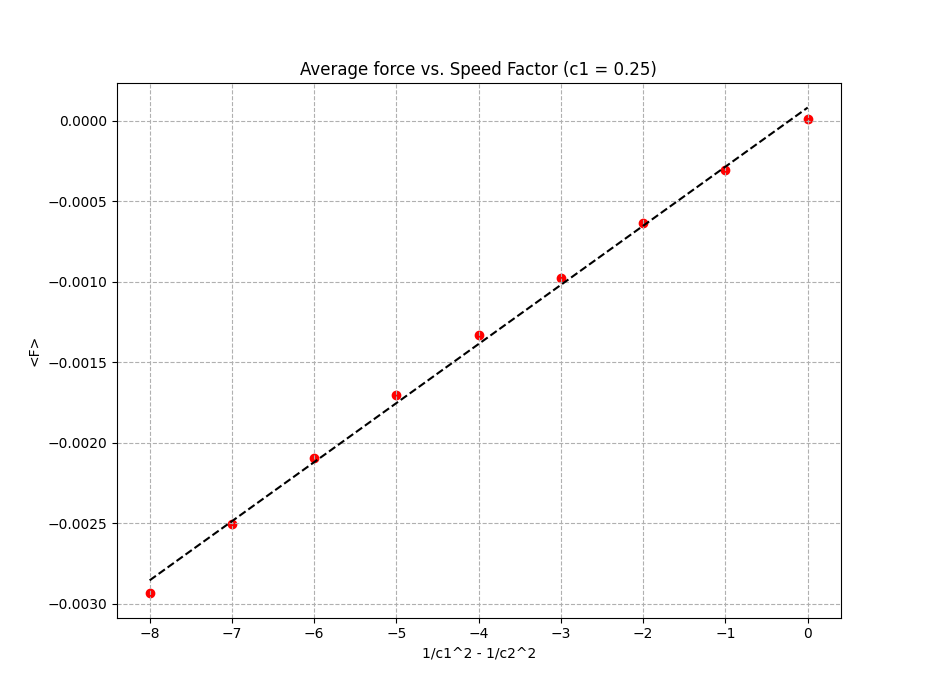
\includegraphics[width=\textwidth]{images/Results/Result_c1_050.png}
    \caption{Relation between the force and wave speed with medium speed $c_1 = 0.5$.}
    \label{fig:wavenumber}
    \end{subfigure}
    \begin{subfigure}{0.4\textwidth}
    \centering
    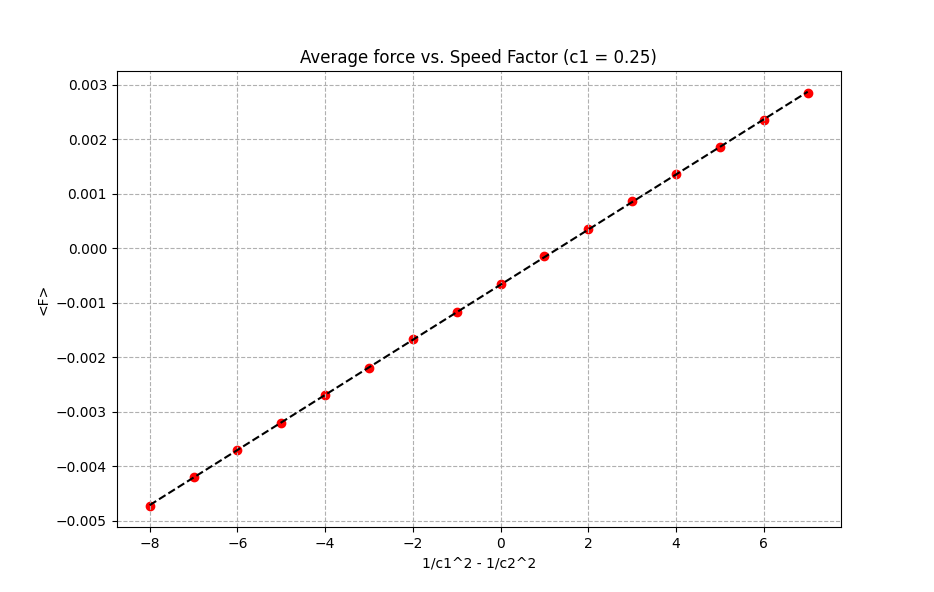
\includegraphics[width=\textwidth]{images/Results/Result_c025_fixed.png}
    \caption{Relation between the force and speed with medium speed $c_1 = 0.25$.}
    \label{fig:amplitude}
    \end{subfigure}
    \caption{Compilation of results of the acoustic radiation force.}
    \label{fig:ARF_results}
\end{figure*}
